\Subsection{Basics}

\begin{definition}\textbf{Stable sorting algorithm}

    The given sorting algorithm is called \textbf{stable} if equal elements are placed in the same order (among these equal elements) as it was in the initial placement, i.e. $\forall i \neq j: a_i = a_j, \ \pi$ - some permutation that sorts the elements, then $i < j \implies \pi(i) < \pi(j)$.

\end{definition}

\begin{definition}\textbf{Inversion}

    Inversion is a pair $(i, \ j)$, s.th.: $i < j: a_i > a_j$.
\end{definition}

\begin{definition}
    $I$ - number of inversions in the array.
\end{definition}

\begin{definition}
    The array is sorted $\Leftrightarrow$ $I = 0$.
\end{definition}

\begin{lemma}

    The sorting algorithm $A$ based on the comparisons of the elements which does $o(n \log{n})$ comparisons for all posible inputs of size $n$ is \textbf{incorrect}, i.e. $\exists$ test $T$ on which the result of sorting by $A$ will be \textbf{incorrect}.

\end{lemma}

\begin{proof}

    Notice that an input of size $n$ can be expressed as a permutation of indicies $\pi: I \to I$ where $I$ is the set of indicies, i.e. $I:=\{0, 1, 2, .., n-1\}$, then there exist $n!$ inputs.

    \begin{center}
        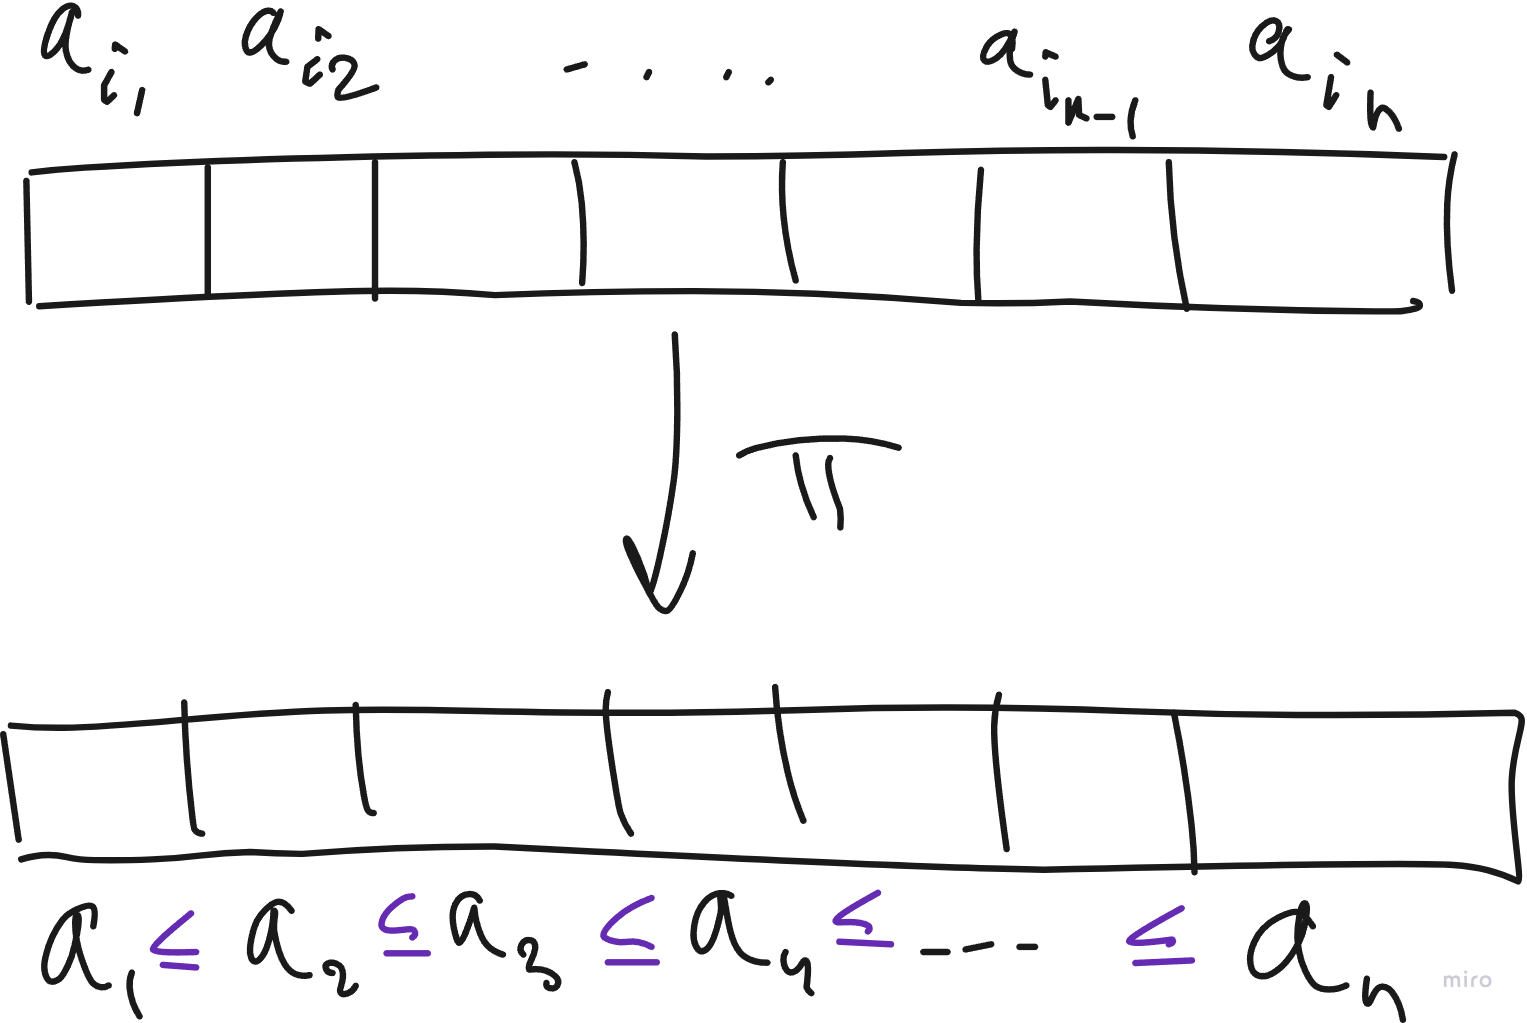
\includegraphics[scale=0.18]{./assets/13-sorting-algorithms/3.png}
    \end{center}

    For the proof it is convinient for us to think that for every input the algorithm $A$ does exactly $k$ comparisons (if in fact it does less then let's just do some meaningless comparisons to get exactly $k$).

    Since the sorting algorithm $A$ is based on comparisons we can assign a binary value for each comparison. The algorithm does $k$ comparisons, if on the $i$-th position the comparison yielded "less or equal" then we assign $0$, if it yielded "greater" we assign $1$ $\implies$ we end up having a binary string of size $k$. Notice that there is a bijection between the set of the produced strings of size $k$ and the set of inputs of size $n$ $\implies$ $2^k = n!$:

    $o(n \log{n}) = \log{2^k} = \log{n!} \implies \log{n!} = o(n \log{n})$ but we know that $\log{n!} = \Theta(n \log{n})$, thus there is a no bijection $\implies$ there exist a test on which the algorithm $A$ produces a wrong result.

\end{proof}


\Subsection{CountSort}

This algorithm sorts a set of integers in range $[0, m)$ in $O(n + m)$ of time and $O(m)$ of memory where $n$ is the size of the input array.

\begin{lstlisting}[language=C++]
int n;
int arr[n];
int count[M] = {0};

for (int i = 0; i < n; ++i) { // O(n)
    count[x]++;
}

for (int x = 0; x < M; ++x) { // O(n + M)
    while(count[x]--) {
        std::cout << x << " ";
    }
}

\end{lstlisting}

Notice that this sorting algorithm is based on the counting not comparisons, thus it is correct and there is a speed boost.


\Subsection{MergeSort: recursive and iterative solutions}

The main idea is to sort the left part, sort the right part and then merge two sorted parts into a single sorted array via two pointers approach.

\Subsubsection{Recursive implementation}

\begin{lstlisting}[language=C++]
void MergeSort(int l, int r, int* a, int* buffer) { // [l, r)
    // base case
    if (r - l <= 1) return;

    int m = (l + r) / 2;
    // sort [l, m)
    MergeSort(l, m, a, buffer);
    // sort [m, r)
    MergeSort(m, r, a, buffer);

    // merge two sorted halves via 2 pointers in O(r - l) time
    Merge(l, m, r, a, buffer);
}
\end{lstlisting}

\textit{buffer} is an additional chunk of memory which is required for the \textbf{Merge} method. The \textbf{Merge} goes through the $[l, m)$ and $[m, r)$ and puts them according to the two pointers technique into the \textit{buffer}.

\begin{lemma}

    Time complexity is $O(n \log{n})$.

\end{lemma}

\begin{proof}
    The recursive formula is as follows: $T(n) = 2 \cdot T(\frac{n}{2}) + n$.

    \underline{Note (Master Theorem)}: $T(n) = a \cdot T(\frac{n}{b}) + n^c$.

    According to the Master Theorem: $a = 2, b = 2, c = 1 \implies a = b^c \implies O(n^c \log{n}) = O(n \log{n})$.

\end{proof}

\Subsubsection{Iterative implementation}

Suppose that the size of the input array is $n = 2^m$ (if not then pad the array with \textbf{MAX\_INT} until it becomes $2^m$). In the recursive approach we traverse the recurse tree from top to bottom, here we traverse it from bottom up. At the bottom we have chunks of size $1$, on the next level chunks of size $2^1$, on the next $2^2$ and so on.

\begin{lstlisting}[language=C++]
int n;
vector<int> arr(n), buffer(n);
// In C++: (1 << k) == 2^k
for (int k = 0; (1 << k) < n; ++k) {
    // iterate through pairs of chunks of size 2^k
    for (int i = 0; i < n; i += 2 * (1 << k)) {
        int m = min(n, i + (1 << k));
        int r = min(n, i + 2 * (1 << k));
        Merge(i, m, r, arr, buffer);
    }
    // now buffer has properly sorted chunks of size 2^(k+1),
    // we need arr to store the updated result after each iteration.
    swap(arr, buffer); // O(1)
}
// the answer is here because we always updated arr inside the for-loop
return arr;

\end{lstlisting}

\begin{center}
    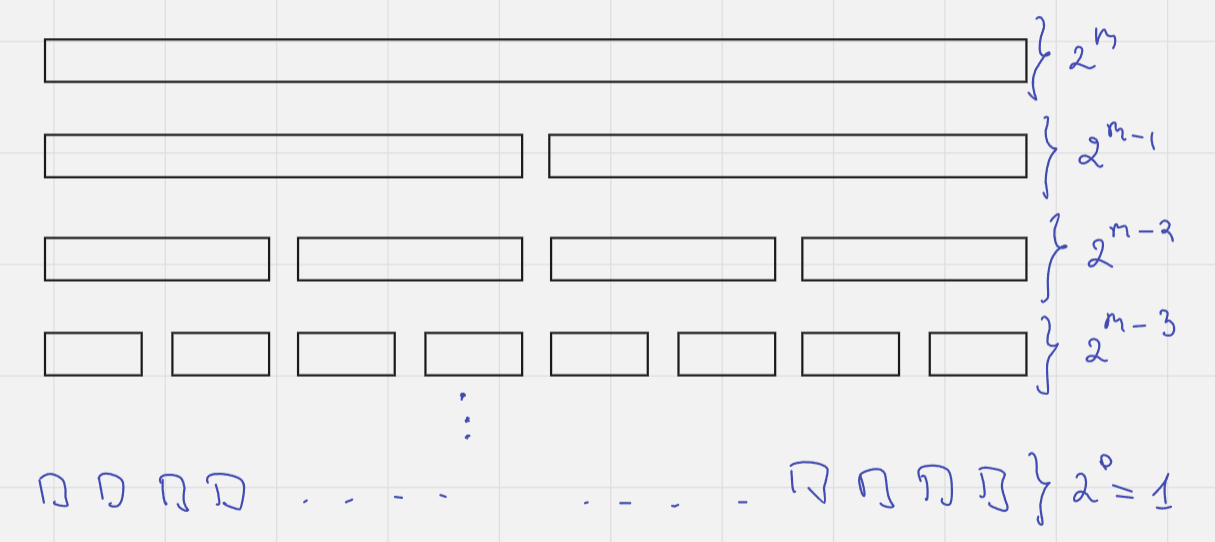
\includegraphics[scale=0.6]{./assets/13-sorting-algorithms/1.PNG}
\end{center}

\Subsection{QuickSort}

\underline{The idea:} select an $x$, split the given array $a$ into 3 parts: $<x$, $=x$, $>x$, then make 2 recursive calls to sort the 1st and the 3rd parts.

\begin{lstlisting}[language=Python]
def QuickSort(a):
    if len(a) <= 1: return a
    x = random.choice(a)
    p1 = select (< x)
    p2 = select (= x)
    p3 = select (> x)
    return QuickSort(p1) + p2 + QuickSort(p3)
\end{lstlisting}

The above is the general idea of the algorithm. In order to make it practically quick the following strategy is used to split the array into 3 parts:

\begin{lstlisting}[language=C++]
void partition(int l, int r, int x, int* a, int &i, int &j) { // [l, r] - both inclusive
    assert(x in a[l..r]); // x must be from a
    i = l;
    j = r;
    while(i <= j) {
        while (a[i] < x) i++;
        while (a[j] > x) j--;
        // a[i] >= x, a[j] <= x => swap elements
        if (i <= j) swap(a[i++], a[j--]);
    }
}
\end{lstlisting}

The above \textit{partition} will split the array into 3 parts $[l, j](j, i)[i, r]$ where:

1. $a[l, j] \leq x$.

2. $a[j+1, i-1] = x$.

3. $a[i, r] \geq x$.

\begin{lemma}
    The algorithm will not exceed the bounds $[l, r]$.
\end{lemma}

\begin{proof}
    $x \in a[l, r] \implies$ there will be at least one \textbf{swap} operation executed (e.g. once $a[i] = x$ and $a[j] = x$). After the last \textbf{swap} the following holds: $l \leq i,\ i \geq j,\ j \leq r$.
\end{proof}

The implementation of the \textbf{QuickSort}:

\begin{lstlisting}[language=C++]
void QuickSort(int l, int r, int* a) { // [l, r] - both inclusive
    if (l >= r) return;
    int i, j;
    int x = a[random in [l, r]];
    // partition accepts i and j by reference and updates them
    Partition(l, r, x, i, j);
    // now: a[l,j] < x, a(j, i) = x, a[i, r] > x
    // we need to sort the 1st and the 3rd parts
    QuickSort(l, j, a); // j < i
    QuickSort(i, r, a); // j < i
}
\end{lstlisting}

\Subsection{Comparison of the sorting algorithms}

\begin{center}
    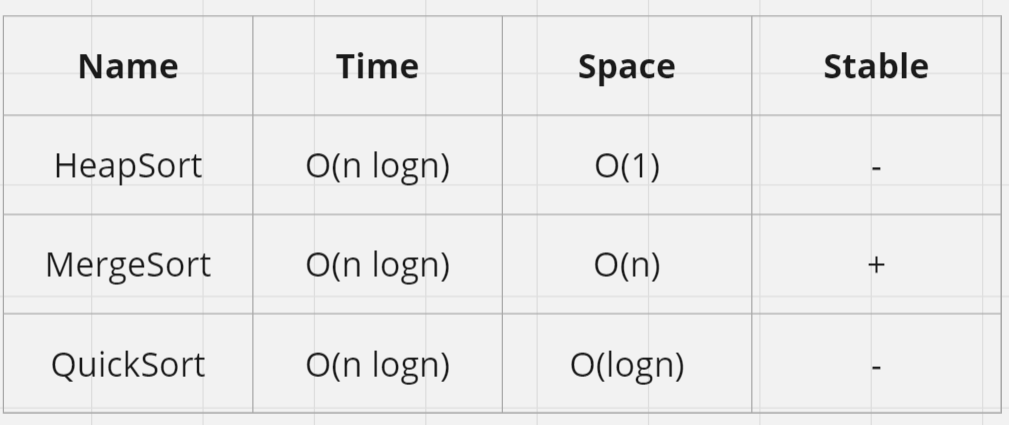
\includegraphics[scale=0.6]{./assets/13-sorting-algorithms/2.PNG}
\end{center}

Notice that among the mentioned sorting algorithms no one is able to make a stable sorting in $O(1)$ of space. There exist such an algorithm, it is implemented via \textbf{inplace stable merge} in $O(n \log{n})$ of time and $O(1)$ of space.

\Subsection{Integer Sorting}

\Subsubsection{Stable CountSort}

Let's take a look at somewhat altered sorting problem: we are given an array of pairs $(a_i,\ b_i)$ of integers and we need to sort in a \textbf{stable} manner.

\begin{lstlisting}[language=C++]
int pos[n] = {0};
int count[m] = {0};

void CountSort(int n, int* a, int* b) { // 0 <= a[i] < m
    for (int i = 0; i < n; ++i) {
        // count the number of occurrences of a[i]
        count[a[i]]++;
    }

    // pos[i] = "position of the start of the chunk which contains pairs <i, ?>"
    pos[0] = 0;
    for (int i = 0; i + 1 < m; ++i) {
        pos[i + 1] = pos[i] + count[i];
    }
    for (int i = 0; i < n; ++i) {
        int index = pos[a[i]]++;
        result[index] = {a[i], b[i]};
    }
}
\end{lstlisting}

Since the algorithm is \textbf{stable} the following algorithm in the next section can be implemented.


\Subsubsection{RadixSort}

Let's sort $n$ strings of length $L$ where symbols of strings are integers in range $[0, k)$.

\textbf{Algorithm}: firstly, sort (via stable sorting algorithm) by the \textbf{last} symbol, then sort by the pre-last symbol, .., sort by the 1st symbol.

\textbf{Correctness}: we are sorting via a stable sorting algorithm some strings by a symbol on the position $i$. In this case, the strings are already sorted by the suffix $(i, L]$. Due to stability of the sorting algorithm, we can state that the strings that have equal $i$-th symbols will be sorted preserving their relative order after previous sorting iteratation, i.e. by the suffix $(i, L]$ $\implies$ the strings are now sorted by suffix $[i, L]$.

\textbf{Time complexity}: $L$ times we call the \textbf{CountSort} algorithm $\implies$ it will sort the strings in $\Theta(L \cdot (n + k))$.

Notice that $\forall b$ - the integer system base, any integer in $[0, m)$ is a string of length $\log_{b}{m}$ over the alphabet $[0, b) \implies$ we can sort integers over base $b$ in $\Theta((n + b) \cdot \lceil \log_{b}{m} \rceil)$. Then once $b = n$ we have the optimum time of $\Theta(n \cdot \lceil \log_{n}{m} \rceil)$.

\underline{The idea of the integer sorting}: we transform integers of the given array from the base of $10$ into the base of $n$ and apply the string sorting algorithm described above.


\Subsubsection{BucketSort}

The idea is to place all of the elements $x$ ($\min \leq x \leq \max$) into $n$ buckets. In order to do that the numeric line is splitted into $n$ segments of equal size where the $i$-th segment contains the elements from the following range:

$L := \max - \min + 1$, $[\min + \frac{i}{n}L, \ \min + \frac{(i+1)}{n}L)$

In this case, each element $x_j$ will be placed into the segment of number $i_j = \lfloor \frac{x_j - \min}{L} \cdot n \rfloor$. The buckets themselves are already sorted, we only need to sort elements inside each bucket. It can be done either by calling the BucketSort recursively or by running any other integer sorting algorithm on each bucket.

\begin{lstlisting}[language=C++]
void BucketSort(vector<int>& a) { // we update the provided array
    if (a.empty()) return;
    int n = a.size();
    int min = min_element(a);
    int max = max_element(a);
    int L = max - min + 1;

    if (min == max) return;
    vector<int> buckets[n]; // array of n vectors

    for (int x : a) {
        int bucketIndex = n * (x - min) / L;
        buckets[bucketIndex].push_back(x);
    }
    a.clear();
    for (int i = 0; i < n; ++i) {
        // sort the i-th bucket
        BucketSort(buckets[i]);
        // place the elements back into a
        for (int x : buckets[i]) {
            a.push_back(x);
        }
    }
}
\end{lstlisting}

\begin{lemma}
    BucketSort works in $O(n \cdot \lceil \log{(\max - \min)} \rceil)$ of time.
\end{lemma}

\begin{proof}
    The algorithm divides the numbers into buckets only if $n \geq 2$, thus the $L$ is being reduced on each recursive call at least by $2$ (in particular, $L \to \frac{L}{n}$) $\implies$ the depth of the recursion is not more than $\log{L}$, each recursion level has not more than $n$ buckets.
\end{proof}